\documentclass[a4paper,12pt]{article}
\usepackage[a4paper,top=1.3cm,bottom=2cm,left=1.5cm,right=1.5cm,marginparwidth=0.75cm]{geometry}
%%% Работа с русским языком
\usepackage{cmap}					% поиск в PDF
\usepackage{mathtext} 				% русские буквы в фомулах
\usepackage[T2A]{fontenc}			% кодировка
\usepackage[utf8]{inputenc}			% кодировка исходного текста
\usepackage[english,russian]{babel}	% локализация и переносы

\usepackage{graphicx}
\usepackage{mathtools}
\usepackage{wrapfig}
\usepackage{tabularx}
\usepackage{amssymb}
\usepackage{hyperref}
\usepackage[rgb]{xcolor}
\hypersetup{colorlinks=true,urlcolor=blue}
\setcounter{secnumdepth}{0}
%% Шрифты
\usepackage{euscript}	 % Шрифт Евклид
\usepackage{amsmath}
\usepackage{mathtools}
%%% Заголовок
\author{Tsvetkova Amelia}
\title{Лабораторная работа по общей физике}

\date{\today}
\begin{document}
\begin{titlepage}
    \newpage
    \begin{center}
    {\large МОСКОВСКИЙ ФИЗИКО-ТЕХНИЧЕСКИЙ ИНСТИТУТ (НАЦИОНАЛЬНЫЙ ИССЛЕДОВАТЕЛЬСКИЙ УНИВЕРСИТЕТ)}
    \vspace{1cm}

    {\largeФизтех-школа аэрокосмических технологий}
    \vspace{6em}
    \end{center}
    
    \vspace{1.2em}

    \begin{center}
    \Large Лабораторная работа №4.3.5 \\
    Изучение голограммы
    \linebreak
    \end{center}
    
    \vspace{11em}
    
    \begin{flushright}
                       {\large Работу выполнила\\
                       Цветкова Амелия Антоновна\\
                       Б03-303 }
    \end{flushright}

    \vspace{\fill}

    \begin{center}
    Долгопрудный, 2025
    \end{center}

    \end{titlepage}

\paragraph{Цель работы:} изучить свойства голограмм точечного источника и объемного предмета.

\paragraph{В работе используются:} гелий-неоновый лазер, голограммы, набор линз, предметная шкала, экран, линейка.

\section{Теоретические сведения}

\subsection{Принципы голографии}

Приёмники света (глаз человека, фотопластинка, фотоэлемент) реагируют на поток энергии световой волны, т. е. величину, пропорциональную квадрату амплитуды. Информация о фазовой структуре волны (т. е. о форме волнового фронта) оказывается при этом утраченной.

Пусть некоторый предмет освещается когерентным светом лазера и пусть волна, отражённая предметом (будем называть её далее предметной волной), создаёт в плоскости \( z = 0 \) световое поле:

\[ f_n(x,y) = a(x,y)e^{i\varphi(x,y)}. \]

Установим в плоскости \( z = 0 \) фотопластинку. Предположим, что функция пропускания фотопластинки после необходимой обработки (проявление, закрепление) пропорциональна интенсивности волны, освещающей пластину во время экспозиции, т. е. пропорциональна величине \( I(x,y) = |a(x,y)|^2 \). Информация о фазовой структуре волны \(\varphi(x,y)\) будет при этом утеряна.

\begin{figure}[h]
\centering
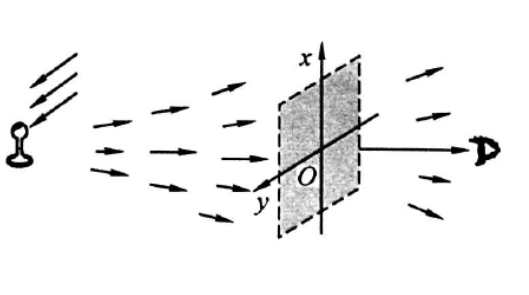
\includegraphics[width=0.2\linewidth]{img2.png}
\caption{Световое поле предмета}
\label{img2}
\end{figure}

\begin{figure}[h]
\centering
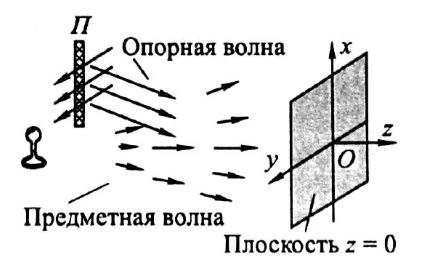
\includegraphics[width=0.2\linewidth]{img3.png}
\caption{Запись голограммы}
\label{img3}
\end{figure}

Следуя идее Габора (1948 г.), изменим схему эксперимента: пусть на фотопластинку кроме предметной волны, создающей на фотопластинке поле \( f_n(x,y) \), падает ещё некоторая волна с известным распределением амплитуд и фаз колебаний \( f_o(x,y) = a_o(x,y)e^{i\varphi_o(x,y)} \), называемая опорной волной. При этом необходимо обеспечить когерентность предметной и опорной волны — волны должны интерферировать. Излучение лазера частично проходит через полупрозрачную пластинку П, освещая предмет, а частично отражается от неё, создавая опорный пучок. Когерентность предметной и опорной волн обеспечивается высокой степенью монохроматичности лазерного излучения (разность хода между предметной и опорной волнами меньше длины когерентности для любой точки фотопластинки).

Суммарное поле на голограмме

\[ f(x,y) = f_n(x,y) + f_o(x,y), \]

а интенсивность (а следовательно, и функция пропускания фотопластинки после необходимой обработки) есть

\[ t(x,y) \propto I(x,y) = |f_n(x,y) + f_o(x,y)|^2. \]

Раскрывая квадрат модуля в полученном выражении

\[ t \propto |f_n|^2 + |f_o|^2 + f_nf_o^* + f_n^*f_o = a^2 + a_o^2 + 2aa_o \cos(\varphi - \varphi_o), \]

убеждаемся, что в функции пропускания (а именно, в слагаемом, связанном с интерференцией опорной и предметной волн) сохранилась информация о фазе предметной волны \(\varphi(x,y)\).

Фотопластинка с зарегистрированным на ней результатом интерференции предметной и опорной волны называются голограммой.

\subsubsection{Голограмма точечного источника (голограмма Габора)}

Для уяснения сути метода рассмотрим в качестве предмета точечный источник света \(S\), т. е. создадим сферическую предметную волну:

\[ f_n = \frac{a_n}{r} e^{ikr}, \]

где \( r = \sqrt{z_0^2 + x^2 + y^2} \) — расстояние от источника \(S\) до точки \((x,y)\) фотопластинки.

В качестве опорной волны возьмём плоскую волну, бегущую вдоль оси \(z\) и падающую нормально на фотопластинку, расположенную в плоскости \( z = 0 \):

\[ f_o = ae^{ikz}, \]

т. е. опорная волна создаёт во всех точках фотопластинки поле одинаковой амплитуды и фазы.

Принимая фазу колебаний в плоскости \( z = 0 \) равной нулю, запишем \( f_0 = a \). Кроме того, для упрощения формул будем далее полагать, что амплитуда сферической волны во всех точках фотопластинки равна амплитуде плоской волны, т. е. \( f_n \approx a e^{ikr} \). Суммарное поле в таком случае имеет вид

\[ f = a e^{ikr} + a. \]

После необходимой фотообработки получаем голограмму с функцией пропускания:

\[ t(x,y) \sim I(x,y) = |a + a e^{ikr}|^2. \]

Мы описали первую стадию голографического процесса — процесс записи голограммы. Теперь необходимо использовать полученную голограмму для восстановления (реконструкции) изображения.

Устанавливаем голограмму в плоскости \( z = 0 \) и освещаем её плоской нормально падающей волной. Для упрощения формул будем считать амплитуду волны равной единице, а фазу без ограничения общности равной нулю, т. е. комплексная амплитуда этой волны (её называют восстанавливающей волной) есть \( f_-(x,y) = 1 \).

Тогда на выходе голограммы, в плоскости, примыкающей к ней справа, получим

\[ f_+(x,y) = f_-(x,y) t(x,y) = |a + a e^{ikr}|^2. \]

Итак, суммарное поле за голограммой описывается действительной положительной функцией. Исследуем его более детально.

\[ f_+(x,y) = 2a^2 + a^2 e^{ikr} + a^2 e^{-ikr} = 2a^2 (1 + \cos(kr)). \]

Поле в плоскости \( z = 0_+ \) представляется в виде суммы трёх слагаемых. Соответственно волна в области \( z > 0 \) есть сумма трёх волн: каждое слагаемое на границе \( z = 0_+ \) ответственно за появление «своей» волны в области \( z > 0 \).

Первое слагаемое \( 2a^2 \) «отвечает» за появление волны \( f_1 = 2a^2 e^{ikz} \) — плоской волны, бегущей в области \( z > 0 \) вдоль оси \( z \). Второе слагаемое \( f_2 = a^2 e^{ikr} \) — волновое поле со сферическим волновым фронтом: именно такое поле создавал в каждой точке плоскости \( z = 0 \) точечный источник света, который находился на расстоянии \( z_0 \) слева от голограммы в процессе записи. Ясно, что и в области \( z > 0 \) поле \( f_2 \) порождает расходящуюся сферическую волну, неотличимую от предметной волны (сферической волны, исходящей из точки \( S \) в процессе записи голограммы). Поэтому наблюдатель, который находится справа (в области \( z > 0 \)) и смотрит на голограмму как в окошко, «увидит в окне» на расстоянии \( z_0 \) слева от голограммы светящуюся точку \( S' \), т. е. расходящаяся сферически волна кажется наблюдателю исходящей из точки \( S' \), хотя никакой светящейся точки на стадии реконструкции изображения нет, — есть только фотопластинка-голограмма, освещаемая плоской волной. Это — мнимое изображение предмета.

Рассмотрим теперь последнее, третье, слагаемое в (3.85): \( f_3 = a^2 e^{-ikr} \). Волновой фронт в этой волне «вывернут наизнанку» по отношению к волне \( f_2 \): если в волне \( f_2 \) колебание в точке \((x,y)\) плоскости \( z = 0 \) отстаёт по фазе от колебаний в начале координат, то в волне \( f_3 \) колебание в точке \((x,y)\) опережает по фазе колебание в начале координат на ту же величину. Это слагаемое описывает поле, которое создавала бы в плоскости \( z = 0 \) сферическая волна, сходящаяся в точку \( S'' \) на расстоянии \( z_0 \) справа (рис. 3.50). Ясно поэтому, что граничное поле \( f_3 \), возникающее в процессе реконструкции, порождает сферическую волну, сходящуюся в точку \( S'' \). Это — действительное изображение предмета. Его можно наблюдать, расположив на расстоянии \( z_0 \) за голограммой экран наблюдения, — мы увидим яркую точку, в которую сфокусирована волна.

Описанные закономерности сохраняются в общих чертах при голографировании произвольного предмета: в процессе реконструкции возникают три волны: волна, создающая мнимое изображение, которое находится слева от голограммы, там же, где находился предмет при записи; волна, создающая действительное изображение, которое располагается симметрично справа от голограммы; а также волна, бегущая вдоль оси \( z \) и не несущая информации о форме волнового фронта предметной волны.

\subsubsection{Зонная решётка Габора}

Вернёмся к интерференционной картине, которая записана на голограмме точечного источника. Используем приближённое выражение

\[ r \approx \sqrt{z_0^2 + x^2 + y^2} \approx z_0 + \frac{x^2 + y^2}{2z_0} = z_0 + \frac{\rho^2}{2z_0}, \]

где \( \rho^2 = \sqrt{x^2 + y^2} \) — расстояние от начала координат до точки \((x,y)\) в плоскости фотопластинки. Соответственно фаза колебаний в сферической волне в точке \( (x,y) \) есть

\[ \varphi = kr \approx kz_0 + \frac{k}{2z_0} \rho^2. \]

Принимая начальную фазу на оси \( z \) в плоскости \( z = 0 \) нулевой, запишем:

\[ \varphi = \frac{k}{2z_0} \rho^2. \]

Мы полагаем, таким образом, что колебания опорной (плоской) волны и сферической волны в точке \( (x = 0, y = 0) \) синфазны. Тогда получим

\[ I(\rho) = 2a^2 \left( 1 + \cos \frac{k\rho^2}{2z_0} \right). \]

Мы видим, что интерференционная картина имеет вид колец, центр которых находится в начале координат. Функция \( I(\rho) \) показана на рис. 3.51. Радиус первого (тёмного) кольца \( \rho_1 \) находим из условия \( k\frac{\rho_1^2}{2z_0} = \pi \) (при этом \( \cos k\frac{\rho_1^2}{2z_0} = -1 \) и \( I(\rho_1) = 0 \)), откуда получаем:

\[ \rho_1 = \sqrt{\lambda z_0}. \]

Вообще радиусы светлых и тёмных колец находятся по формуле

\[ \rho_m = \sqrt{m\lambda z_0} \]

(при \( m \) нечётном — тёмные кольца, при \( m \) чётном — светлые), которая совпадает с выражением, определяющим радиусы тёмных и светлых колец в зонной пластинке Френеля.

Отличие состоит в том, что в нашем случае переход от светлых колец к тёмным происходит плавно. Интерференционная картина (голограмма точечного источника) называется зонной решёткой Габора. Как следует из проведённого выше анализа, зонная решётка Габора работает одновременно и как собирающая линза (фокусируя параллельный пучок света в точку \( S'' \) — действительный фокус зонной пластинки), и как рассеивающая линза, которая преобразует параллельный пучок, падающий на пластинку, в расходящуюся сферическую волну, исходящую из мнимого фокуса \( S' \), и как плоскопараллельная пластинка, поскольку часть света за пластинкой сохраняет структуру освещающего параллельного пучка.

\subsubsection{Сферическая восстанавливающая волна}

Рассмотрим ещё одно свойство голограммы точки. Пусть восстанавливающая волна является не плоской, а сферической, расходящейся от точки, расположенной на расстоянии \( z_1 > z_0 \) от голограммы. Используя параболическое приближение, запишем комплексную амплитуду падающей волны в плоскости голограммы:

\[ f_-(\rho) = e^{-i \frac{k}{2z_1} \rho^2}. \]

Восстановленное поле в плоскости \( z = 0 \):

\[ f_+(\rho) = f_-(\rho) t(\rho). \]

Используя (3.89) и (3.83), получим (с точностью до несущественных констант)

\[ f_+(\rho) = e^{-i \frac{k}{2z_1} \rho^2} + e^{-i \frac{k}{2} \left( \frac{1}{z_1} + \frac{1}{z_0} \right) \rho^2} + e^{-i \frac{k}{2} \left( \frac{1}{z_0} - \frac{1}{z_1} \right) \rho^2}. \]

Из этого выражения видно, что расстояние \( b_2 \) от голограммы до мнимого изображения источника уменьшается, так как

\[ \frac{1}{b_2} = \frac{1}{z_0} + \frac{1}{z_1}, \]

т. е. это изображение приближается к голограмме. В то же время расстояние \( b_3 \) от голограммы до действительного изображения увеличивается:

\[ \frac{1}{b_3} = \frac{1}{z_0} - \frac{1}{z_1}. \]

Это свойство голограммы следует иметь в виду при объяснении изменения масштабов изображений трёхмерного предмета при освещении голограммы сферической волной.

В случае произвольного предмета на голограмме записывается сложный интерференционный узор, который можно рассматривать как совокупность зонных кольцевых решёток Габора, причём каждая из них ответственна за восстановление «своей» точки предмета на стадии реконструкции изображения.

\subsubsection{Разрешающая способность голограммы}

Рассмотрим более детально волну, ответственную за создание действительного изображения. Конечно, сходящаяся сферическая волна не фокусируется строго в точку \( S'' \): изображением является не точка, а маленькое дифракционное пятнышко. Действительно, плоская восстанавливающая волна, пройдя сквозь голограмму, преобразуется в сферическую волну (мы говорим сейчас о той части волны, которая ответственна за создание действительного изображения), причём сферический волновой фронт ограничен размерами голограммы. Эта сходящаяся сферическая волна не отличается от сферической волны, возникающей за собирающейся линзой, размер \( D \) которой равен размеру голограммы. При фокусировке света линзой возникает дифракционное пятно Эйри. Ясно, что и голограмма создаёт изображение — дифракционное пятно, размер которого определяется аналогичной формулой:

\[ \Delta x \sim \frac{\lambda}{D} z_0, \]

где \( z_0 \) — расстояние от точечного источника до голограммы в процессе записи, \( D \) — размер голограммы. Если записывать на голограмму изображения двух точек, расстояние между которыми меньше \(\Delta x\), то при восстановлении изображений возникают два пятна, налагающиеся друг на друга так, что, согласно критерию Рэлея, они оказываются неразрешимыми. Сказанное касается, разумеется, и мнимого изображения точечного источника: наблюдателю оно кажется маленьким пятнышком размера \(\Delta x\), находящимся на расстоянии \( z_0 \) за голограммой.

Важнейшее свойство голограммы состоит в том, что любой её малый участок содержит информацию обо всем объекте: ведь поле в каждой точке голограммы является суперпозицией полей, посылаемых всеми точками предмета (и опорной волной). Другими словами, интерференционная картина на каждом небольшом участке голограммы содержит информацию об амплитуде и фазе колебаний всех точек предмета, поэтому изображение может быть восстановлено с помощью небольшого осколка голограммы, полученной при записи. Разумеется, разрешающая способность определяется размером осколка.\footnote{В реальной голограмме разрешающая способность дополнительно ограничивается такими факторами, как разрешающая способность фотоплёнки (зернистость), засветка голограммы сторонними источниками (пятна) и пр.}

\subsubsection{Схема с наклонным опорным пучком}

При наблюдении голографических изображений, полученных по схеме Габора, действительное и мнимое изображения создают взаимные помехи: изображения \( S' \) и \( S'' \) находятся на одной прямой с точкой, в которой расположен глаз наблюдателя. Помехи создаются также возникающей при восстановлении плоской волной, бегущей вдоль оси \( z \) и не несущей информации об объекте. В 1962 году Лейт и Упатниекс предложили использовать для записи голограммы наклонный опорный пучок.

Проследим, каким образом введение опорного наклонного пучка обеспечивает возможность независимого (без взаимных помех) наблюдения действительного и мнимого изображений. «предметом» является «точечный источник» S. Наклон опорного пучка обеспечивается призмой П. Поле предметной волны на голограмме есть

\[ f_n(x,y) = ae^{i\frac{k}{2z_0}(x^2+y^2)} \]

(мы вновь используем параболическое приближение). Наклонная опорная волна имеет вид \( f_0 = ae^{iu_0 x} \), где \( u_0 = k \sin \alpha \) — пространственная частота опорной волны. Мы полагаем, что волны имеют равные амплитуды и создают в начале координат плоскости \( z = 0 \) (плоскость голограммы) синфазные колебания. Функция пропускания проявленной голограммы, пропорциональная интенсивности суммарной волны при записи, имеет вид

\[ t(x,y) \sim \left| ae^{iu_0 x} + ae^{i\frac{k}{2z_0}(x^2+y^2)} \right|^2. \]

Предоставляем читателю убедиться, что слагаемые, ответственные за появление действительного и мнимого изображения при восстановлении, можно записать в виде:

\[ f_3(x,y) \sim be^{i\frac{k}{2z_0}((x+z_0 \sin \alpha)^2+y^2)}, \quad f_4(x,y) \sim be^{-i\frac{k}{2z_0}((x+z_0 \sin \alpha)^2+y^2)}, \]

где \( b \) — комплексная константа. Выражение \( f_3(x,y) \) представляет собой поле, которое создавал бы в плоскости \( z = 0 \) точечный источник, находищийся в точке с координатами \( x_0 = -z_0 \sin \alpha, \, y = 0 \), на расстоянии \( z_0 \) слева от голограммы. Это мнимое изображение предмета \( S' \) (рис. 3.54). Соответственно \( f_4(x,y) \) описывает поле сходящейся в точку \( S'' \) сферической волны. Эта точка находится справа от голограммы на расстоянии \( z_0 \) и смещена относительно оси \( z \) на расстояние \( x_0 = -z_0 \sin \alpha \). Это действительное изображение. Мы видим, что введение наклонного опорного пучка приводит к сдвигу мнимого и действительного изображений таким образом, что наблюдатель может рассматривать их из разных положений (1 и 2 на рис. 3.54), в которых они не создают взаимных помех. Разумеется, угол наклона опорного пучка \( \alpha \) (т. е. его пространственная частота) должен быть выбран правильно: чем шире пространственный спектр предметной волны, тем больше должен быть угол наклона опорного пучка, при котором волны, ответственные за создание действительного и мнимого изображений, не создают взаимных помех.


\section{Экспериментальная установка}

В работе исследуются голограммы точечного источника и трехмерного объекта. Эти голограммы записаны на фотопластинках типа ЛОИ-2, имеющих высокое разрешение: $\sim$ 5000 линий/мм. При записи был использован He-Ne-лазер с длиной волны излучения $\lambda$=632,8нм.

\begin{figure}[h]
\centering
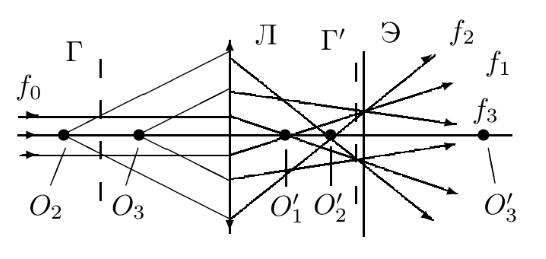
\includegraphics[width=0.8\linewidth]{img1.png}
\caption{Схема установки: Г - голограмма точечного источника}
\label{img1}
\end{figure}

В работе требуется определить расстояние $d$ между голлограммой и точечным источником света. Это расстояние можно считать, измерив радиусы $\rho$ нескольких колец:
\begin{equation}
    p_m=\sqrt{m\lambda z_0}=\sqrt{m\lambda d}
\end{equation}
но их размеры слишком малы, поэтому требуется получить увеличенное изображение. Оно получается при помощи короткофокусной линзы на экране (рис. $\ref{img1}$).

При просвечивании голограммы Г точечного источника плоской волной с амплитудой $f_0=$const, на выходе имеются три волны: плоская с амплитудой $f_1=$const, расходящаяся сферическая $f_2 \propto e^{ikr}$, отвечающая мнимому изображению $O_2$, и сходящаяся сферическая волна $f_3 \propto e^{-ikr}$, отвечающая действительному изображению $O_3$. После прохождения линзы Л волна $f_1$ собирается в фокусе линзы в точке $O'_1$, волны $f_2$ и $f_3$ фокусируются соотвественно в точках $O'_2$ и $O'_3$. Изображение, возникающее на экране Э, можно рассматривать как результат интерференции сферических волн от трех точечных источников: $O'_1, O'_2, O'_3$. Поэтому картина концетрических колец возникает на экране не только тогда, когда на нем образуется изображение $\text{Г}'$ голограммы, но и при многих других положениях линзы. 

Таким образом, чтобы определить радиусы колец, следует убедиться, что на экране действительно возникло изображение голограммы, т.е. плоскости Г и $\text{Г}'$ сопряжены. Для этого вместо голограммы помещают прозрачную предметную шкалу, на которую нанесен тонкий крест с делениями. В этом случае увеличенное изображение креста получается при единственном положении линзы для определенного расстояния между предметом и экраном.

Предметная шкала и голограмма точечного источника смонтированы на платформе в единую плоскую кассету транспарантов. Такая же предметная шкала, закрепленная в отдельной оправе, используется в качестве предмета при определении фокусного расстояния голографической линзы.

Кроме голограммы точечного источника в работе исследуется голограмма объемного предмета. Предмет представляет собой горизонтально расположенную миллиметровую линейку, за которой расположен вертикальный металлический стержень. При записи голограммы предмет располагался на расстоянии 10 см от пластинки. Фотопластинка была обращена к предмету той стороной, на которую нанесена эмульсия. Голограмма установлена в оправе вертикально и может поворачиваться вокруг вертикальной оси. Для измерения угла поворота служит транспортир, закрепленный под голограммой в горизонтальной плоскости.

Источником света служит лазер с диаметром луча < 1мм. В опытах с объемной голограммой требуются более широкие световые пучки. Для расширения пучка используются две линзы: короткофокусная - с фокусным расстоянием < 2 мм и длиннофокусная - с фокусным расстоянием $\sim$ 8 см. Собранный из этих линз расширитель создает пучок диаметром 4-5 см.

\section{Ход работы}
\subsection{Изучение характеристик голограммы точечного источника}
\begin{enumerate}
    \item Настраиваем установку

    Определив расстояние $\Delta x$ между дифракционными максимума на экране и расстояние $L$ от шкалы до экрана, рассчитаем цену деления $D$:
    $$
    \Delta x=(6\pm1)\text{мм} \quad L= (106\pm1)\text{см}
    $$
    $$
    \lambda/D=\Delta x/L \Longrightarrow D=\frac{\lambda L}{\Delta x}=9.40\cdot 10^{-5}\text{м, }
    \sigma_D=9.40\cdot10^{-5}\cdot\sqrt{\Big(\frac{1}{6}\Big)^2+\Big(\frac{1}{106}\Big)^2}=1.57\cdot10^{-5}\text{ м.}
    $$
    \item Определив цену деления той же шкалы, используя линзу с фокусным расстоянием $f=43$см: получим в центре экрана увеличенное изображение предметной шкалы с четкими делениями.

    Измерим расстояния от линзы до предметной шкалы $a$ и до экрана $b$ и рассчитаем увеличение системы. Определим расстояние $D'$ между изображениями штрихов и рассчитаем цену деления $D$ предметной шкалы. 
    $$
    a=(41\pm1)\text{мм}, \quad b=(112.5\pm.5)\text{см}
    $$
    $$
    D'=14/6=2.3\text{мм}
    $$
    $$
    D=\frac{D'\cdot a}{b}=8.38\cdot 10^{-5}\text{м},\quad \sigma_D=8.38\cdot10^{-5}\cdot\sqrt{\Big(\frac{1}{14}\Big)^2+\Big(\frac{1}{41}\Big)^2+\Big(\frac{0.5}{112.5}\Big)^2}=0.63\cdot10^{-5}\text{ м.}
    $$
    $$
    \text{Г}=\frac{b}{a}=27.4, \quad \sigma_\text{Г}=\text{Г}\cdot\sqrt{\Big(\frac{\sigma_a}{a}\Big)^2+\Big(\frac{\sigma_b}{b}\Big)^2}=0.7
    $$

    \item Получили на экране изображение голограммы точечного источника. Прикладываем к экрану лист бумаги, отмечаем на нем радиусы нескольких темных колец и измеряем эти радиусы линейкой. Зная увеличение системы, рассчитаем размеры колец на голограмме, а затем определим расстояние $d$ от голограммы до точечного источника, который был использован при ее создании.

    \begin{table}[h!]
    \centering
    \begin{tabular}{||c|c|c|c|c|c|c|c|c|c||}
    \hline
        $m$ & 1 & 2 & 3 & 4 & 5 & 6 & 7 & 8 & 9 \\
        \hline
        $r_m,$мм & 2.5 & 4.5 & 6.0 & 7.0 & 8.0 & 9.0 & 10.0 & 11.0 & 11.5 \\
        \hline
        $\sigma_{r_m},$мм & 1 & 1 & 1 & 1 & 1 & 1 & 1 & 1 & 1 \\
        \hline
        $r_m^{\text{ист}},$мм & 0.091 & 0.164 & 0.219 & 0.2556 & 0.292 & 0.329 & 0.365 & 0.402 & 0.420 \\
        \hline
        $\sigma_{r_m^{\text{ист}}},$мм & 0.004 & 0.004 & 0.004 & 0.004 & 0.004 & 0.004 & 0.004 & 0.004 & 0.004 \\
        \hline
        ${r_m^{\text{ист}}}^2,\text{мм}^2$ & 0.008 & 0.027 & 0.049 & 0.065 & 0.085 & 0.108 & 0.133 & 0.161 & 0.176 \\
        \hline
        $\sigma_{{r_m^{\text{ист}}}^2}^2,\text{мм}^2$ & 0.0007 & 0.0012 & 0.0016 & 0.0019 & 0.0021 & 0.0024 & 0.0027 & 0.0029 & 0.0031 \\
    \hline
    \end{tabular}
    \end{table}

    \begin{figure}[h]
    \centering
    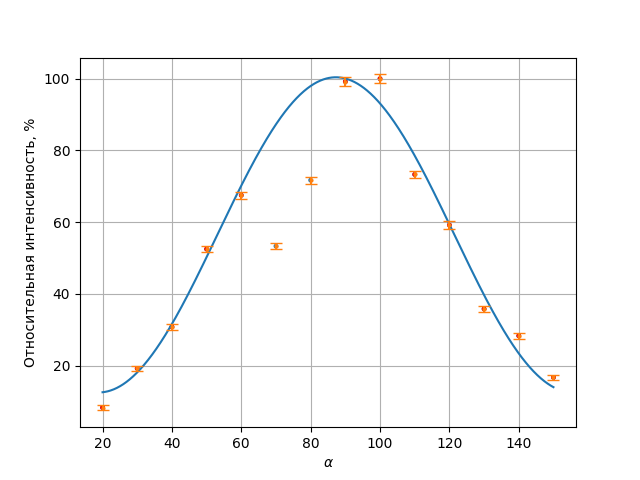
\includegraphics[width=1\linewidth]{graph1.png}
    \caption{Зависимость $r_m^2(m)$}
    \label{graph1}
    \end{figure}
    
    $$
    d=\frac{r_m^2}{m\lambda}=\frac{k}{\lambda}=\frac{0.0107\cdot 10^{-6}}{532\cdot 10^{-9}}=20.11\text{мм}
    $$
    $$
    \sigma_{d} = d\sqrt{\left(\frac{\sigma_k}{k}\right)^2+\left(\frac{\sigma_\text{Г}}{\text{Г}}\right)^2}=20.11\cdot\sqrt{\left(\frac{0.0005}{0.0107}\right)^2+\left(\frac{0.7}{27.4}\right)^2}=1.07\text{vм}
    $$
    
    \begin{center}
        \boxed{d_1=(20.11\pm1.07)\text{мм}(\varepsilon=5.32\%)}
    \end{center}

    \item Перемещая линзу вдоль луча, получим на экране сначала изображение мнимого $O_2$, а затем действительного $O_3$ точечного источника. Для каждого изображения измерим необходимые геометрические размеры установки и, зная фокусное расстояние линзы, рассчитаем расстояния от точечных источников до голограммы.

    для мнимого $O_2$:
    $$
    a=(57\pm3)\text{мм}, \quad b=(190\pm3)\text{мм}
    $$
    $$
    d_2=28.1\text{мм}, \quad \sigma_{d_2}=28.1^2\cdot\sqrt{\Big(\frac{3}{190^2}\Big)^2+\Big(\frac{3}{57^2}\Big)^2}=0.7\text{мм}
    $$

    для действительного $O_3$:
    $$
    a=(36\pm1)\text{см}, \quad b=(115\pm3)\text{мм}
    $$
    $$
    d_3=34.2\text{мм}, \quad \sigma_{d_3}=34.2^2\cdot\sqrt{\Big(\frac{3}{115^2}\Big)^2+\Big(\frac{10}{360^2}\Big)^2}=1.0\text{мм}
    $$

    \item Снова получим на экране изображение голограммы. Перемещая кассету перпендикулярно оптической оси, смещаем голограмму ближе к границе светового пятна. Опять получим изображения действительного и мнимого источников и определим их расстояния до голограммы.

    для мнимого $O_2$:
    $$
    a=(44\pm3)\text{мм}, \quad b=(125\pm3)\text{мм}
    $$
    $$
    d_4=26.3\text{мм}, \quad \sigma_{d_4}=26.3^2\cdot\sqrt{\Big(\frac{3}{125^2}\Big)^2+\Big(\frac{3}{44^2}\Big)^2}=0.2\text{мм}
    $$

    для действительного $O_3$:
    $$
    a=(35\pm1)\text{см}, \quad b=(135\pm3)\text{мм}
    $$ 
    $$
    d_5=36.0\text{мм}, \quad \sigma_{d_5}=36.0^2\cdot\sqrt{\Big(\frac{3}{135^2}\Big)^2+\Big(\frac{10}{350^2}\Big)^2}=1.1\text{мм}
    $$

    \item Добиваемся полного разделения пучков света на удаленном экране. По размерам световых пятен определяем, что правое маленькое пятно, в котором видна шкала, соответствует действительному изображению, левое - мнимому.
    \item Перед голограммой поставим предметную шкалу, закрепленную в отдельной оправе. Получим в одном из пятен резкое изображение делений крестообразной шкалы. 
    
    Измерим расстояние между штрихами $D'$ на экране и расстояние $b$ от экрана до голограммы:
    $$
    D'=12/4=3\text{мм}, \quad b=(106\pm 3)\text{см}
    $$
    Используя эти данные, а также найденную ранее цену деления шкалы $D$, рассчитаем фокусное расстояние голографической шкалы:
    
    $$
    f=\frac{b\cdot D}{D'}=31.8\text{мм}, \quad \sigma_f=31.8\cdot\sqrt{\Big(\frac{3}{106}\Big)^2+\Big(\frac{1}{12}\Big)^2+\Big(\frac{0.63}{8.38}\Big)^2}=3.9\text{мм}
    $$
    
\end{enumerate}

\subsection{Изучение характеристик голограммы объемного предмета}
\begin{enumerate}
    \item Собираем на оптическом столе расширитель пучка.
    \item Установим короткофокусную линзу. Перемещая ее в плоскости, перпендикулярной лучу, вновь совмещаем центр светового пятна с его первоначальным положением.
    \item Добиваемся, чтобы из собранного расширителя выходил параллельный пучок: при полном заполнении светом длиннофокусной линзы диаметр светового пятна на удаленном экране равен диаметру линзы, при неполном - можно контролировать размер пятна, перемещая вдоль луча переносной экран.
    
    \item Помещаем голограмму в расширенный пучок лазера фотоэмульсией к лазеру и находим мнимое изображение предмета. Для этого располагаемся за экраном с правой стороны. Медленно поворачивая голограмму вокруг вертикальной оси и перемещая глаз в горизонтальной плоскости на высоте луча, находим изображение линейки в окне голограммы.
    \item По углу поворота голограммы оценим угол падения опорной волны, который был выбран при получении голограммы:
    $$
    \alpha=45^\circ\pm5^\circ
    $$
    \item Постепенно закрывая голограмму листом бумаги, убедимся в том, что изображение предмета восстанавливается даже по небольшой части голограммы. 
    
    Объясним это явление. В отличие от фотографии, где каждая точка соответствует конкретной точке объекта, на голограмме каждая точка содержит свет от всех точек объекта, закодированный в интерференционных полосах. При освещении голограммы опорной волной, её микроструктура работает как дифракционная решетка, воссоздавая исходную волновую фронт объекта. Даже маленький фрагмент голограммы способен дифрагировать свет так, чтобы восстановить целое изображение (хотя и с меньшим разрешением). Физическая основа явления: принцип Гюйгенса-Френеля: каждая точка волнового фронта (в данном случае — фрагмент голограммы) действует как источник вторичных волн, которые вместе восстанавливают полную картину.
    \item Оценим расстояние от линейки до вертикального стержня, расположенного за ней, фиксируя по транспортиру угол, под которым наблюдается изображение.

    $$
    \varphi_1=90^\circ\pm5^\circ, \quad l_1=195.2
    $$
    $$
    \varphi_2=110^\circ\pm5^\circ, \quad l_2=194.5
    $$

    Теперь оценим расстояние от стержня до линейки:
    $$
    h=\frac{l_2-l_1}{\frac{1}{\tan{\varphi_1}}-\frac{1}{\tan{\varphi_2}}}=1.92\text{см}
    $$
    \item Проводим наблюдение мнимого изображения предмета, используя в качестве лупы линзу с фокусным расстоянием 20 см.

    \item Находим действительное изображение: голограмма должна при этом располагаться перпендикулярно падающему пучку света, глаз наблюдателя - с левой стороны от экрана на расстоянии от пластинки 50-80 см Поскольку это изображение расположено между пластинкой и глазом, удобно рассматривать его через лупу.

    По мере удаления лупы от глаза мы сначала видим резкое изображение стержня и только потом - линейки.

    Объясним это явление. Голограмма восстанавливает действительное изображение стержня перед собой, создавая отдельный волновой фронт, который фокусируется ближе к наблюдателю, чем сама пластинка с линейкой. При удалении лупы сначала теряется резкость стержня (из-за малой глубины резкости ближнего изображения), а затем линейки (как протяжённого объекта с большей глубиной резкости).

    \item Повернем голограмму на $180^\circ$ вокруг вертикальной оси (фотоэмульсией от лазера). Найдем действительное и мнимое изображения.

    Заметим, что они поменялись местами: теперь действительное наблюдается под углом $45^\circ$ справа против хода луча.
    \item Снова развернем голограмму эмульсией к лазеру. При перемещении короткофокусной линзы расширителя вдоль луча мнимое изображение не меняется. Масштаб действительного изображения увеличивается при приближении линзы к голограмме.

    Объясним это явление. При перемещении линзы вдоль луча мнимое изображение остаётся неизменным, так как его положение определяется только углом падения опорной волны и структурой голограммы. Действительное же изображение увеличивается при приближении линзы к голограмме, потому что линза изменяет расходимость восстанавливающего пучка, что эквивалентно изменению масштаба реконструкции — это прямое следствие голографического принципа сохранения угловых соотношений при изменении параметров освещения.
\end{enumerate}

\section{Выводы}
В данной лабораторной работе мы изучили голограмму точечного источника и определили несколькими способами расстояние до записанного на нее точечного источника. Кроме того, мы изучили фокусирующие свойства голограмм точечного источника и исследовали некоторые особенности голограмм объемного объекта.

\section{Приложение}

\subsection{Запись толстослойной голограммы}
Если голограмма записана на фотопластинке с толстым слоем эмульсии и при большом угле падения опорной волны, то она регистрирует объёмную картину интерференции предметной и опорной волн. Будем считать, что предметная волна с комплексной амплитудой $f_{\text{пр}}(\mathbf{r})$, где $\mathbf{r} = (x, y, z)$, распространяется в плоскопараллельном слое эмульсии толщины $h$ ($0 \leq z \leq h$). При записи голограммы опорная волна была плоской, её волновой вектор $\mathbf{k}_{\text{оп}}$ лежал в плоскости $(x, z)$ и составлял угол $\alpha$ с осью $z$. Запишем комплексную амплитуду этой волны в виде:

$$
f_{\text{оп}}(\mathbf{r}) = a_{\text{оп}} e^{-i(\mathbf{k}_{\text{оп}} \mathbf{r})} = a_{\text{оп}} e^{-ik(x \sin \alpha + z \cos \alpha)},
$$

где $k$ — волновое число.

После экспонирования фотопластинки и её химической обработки в фотоэмульсии образуются кристаллы металлического серебра, локальная концентрация которых пропорциональна интенсивности интерференционной картины:

$$
|f_{\text{пр}}(\mathbf{r}) + f_{\text{оп}}(\mathbf{r})|^2.
$$

Рассмотрим структуру эмульсии в случае, когда предметная волна является плоской волной с волновым вектором, перпендикулярным плоскости фотопластинки:

$$
f_{\text{пр}}(\mathbf{r}) = a_{\text{пр}} e^{-ikz}.
$$

Интенсивность интерференционной картины:

$$
I(\mathbf{r}) = |a_{\text{пр}}|^2 + |a_{\text{оп}}|^2 + 2|a_{\text{пр}}||a_{\text{оп}}|\cos\left[k((1 - \cos\alpha)z - x \sin\alpha] + \varphi\right),
$$

где $\varphi$ — постоянная разность фаз между предметной и опорной волнами. Отсюда видно, что в рассматриваемом случае линиями постоянной интенсивности являются прямые. В частности, интенсивность максимальна, если:

$$
z = \frac{x}{\tan(\alpha/2)} + \frac{2\pi n - \varphi}{k(1 - \cos\alpha)}, \quad n = 0, \pm 1, \pm 2, \ldots
$$

(здесь использовано $\tan \alpha/2 = (1 - \cos \alpha)/\sin \alpha$). Кроме того, при постоянной координате $z$ интенсивность периодически меняется вдоль координаты $x$ с периодом:

$$
\Delta x = \frac{\lambda}{\sin \alpha},
$$

где $\lambda$ — длина волны света. На рис. 5а показано семейство прямых, вдоль которых интенсивность интерференционной картины постоянна. Эти прямые параллельны биссектрисе угла между волновыми векторами предметной и опорной волн.

\begin{figure}[h]
\centering
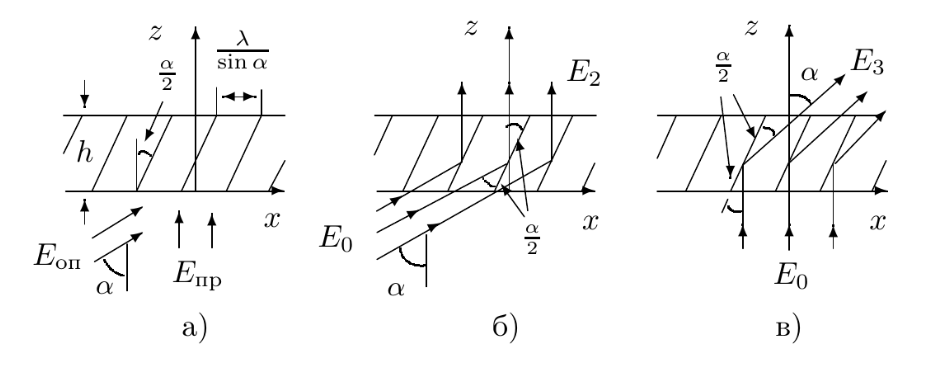
\includegraphics[width=0.8\linewidth]{img4.png}
\caption{Запись и восстановление фронта плоской волны}
\label{img4}
\end{figure}
    
\subsection{Структура эмульсии}
Пропорционально интенсивности $I(\mathbf{r})$ меняется локальная концентрация металлического серебра. Можно сказать, что в рассматриваемом случае эмульсия голограммы представляет собой периодическую последовательность наклонно расположенных зеркал, причём коэффициент пропускания и отражения зеркал меняется вдоль координат $(x, z)$. Эмульсию можно считать тонкой, если проекция $h \tan(\alpha/2)$ ($h$ — толщина эмульсии) линейного размера отдельного зеркала на ось $x$ много меньше периода следования зеркал $\Delta x$, т.е.:

$$
h \tan \frac{\alpha}{2} \ll \frac{\lambda}{\sin \alpha}
$$

или

$$
2 \frac{h}{\lambda} \sin^2 \frac{\alpha}{2} \ll 1.
$$

Толщина эмульсии на фотопластинках ЛОИ-2, используемых в работе:

$$
h \simeq (7 \div 10) \lambda \simeq 5 \, \text{мкм} \quad (\lambda \simeq 0,6 \, \text{мкм}).
$$

При регистрации голограммы точечного источника опорная волна падает на фотопластинку нормально, а угол падения предметной волны на периферии голограммы (в районе десятого интерференционного кольца) $\alpha \simeq 10^{-2}$. Поэтому:

$$
\frac{2h}{\lambda} \sin^2 \frac{\alpha}{2} \simeq 10^{-3},
$$

и эту голограмму можно считать тонкой. Для голограммы предмета угол падения опорной волны $\alpha \simeq 40^\circ$, и тот же параметр достигает значения $\simeq 2$. В этом случае эмульсию следует считать толстой.

\subsection{Условия восстановления изображений}
Рассмотрим условия восстановления действительного и мнимого изображений для толстослойной голограммы. Пусть на голограмму падает плоская волна, волновой вектор $\mathbf{k}_0$ которой лежит в плоскости $(x, z)$ и составляет угол $\beta$ с осью $z$. Комплексная амплитуда этой волны:

$$
f_0(\mathbf{r}) = a_0 e^{-i\mathbf{k}_0 \mathbf{r}} = a_0 e^{-ik(x \sin \beta + z \cos \beta)}.
$$

Падающая волна, проходя через эмульсию голограммы, будет частично рассеиваться на центрах восстановленного серебра. Можно считать, что небольшая область эмульсии вблизи точки $\mathbf{r} = (x, y, z)$ является источником вторичной (рассеянной) волны. Амплитуда вторичной волны пропорциональна концентрации металлического серебра, которая в свою очередь пропорциональна интенсивности интерференционной картины предметной и опорной волн при записи голограммы, а фаза определяется фазой падающей волны. Исходя из этого, запишем комплексную амплитуду волны $f$, рассеянной в точке $\mathbf{r}$ в виде:

$$
f(\mathbf{r}) \sim |f_{\text{пр}} + f_{\text{оп}}|^2 f_0 = f_1(\mathbf{r}) + f_2(\mathbf{r}) + f_3(\mathbf{r}),
$$

где

$$
f_1(\mathbf{r}) = a_0 \left( |a_{\text{оп}}|^2 + |f_{\text{пр}}(\mathbf{r})|^2 \right) e^{-i\mathbf{k}_0 \mathbf{r}}
$$
$$
f_2(\mathbf{r}) = a_0 a_{\text{оп}} f_{\text{пр}}(\mathbf{r}) e^{-i(\mathbf{k}_0 - \mathbf{k}_{\text{оп}}) \mathbf{r}}
$$
$$
f_3(\mathbf{r}) = a_0 a_{\text{оп}} f_{\text{пр}}^{*}(\mathbf{r}) e^{-i(\mathbf{k}_0 + \mathbf{k}_{\text{оп}}) \mathbf{r}}.
$$

Обычно $|a_{\text{оп}}|^2 \gg |f_{\text{пр}}(x, y)|^2$, поэтому $f_1$, как и в случае тонкой голограммы, описывает комплексную амплитуду прошедшей волны. Эта волна распространяется под тем же углом $\beta$, что и падающая. Слагаемое $f_2(\mathbf{r})$ пропорционально комплексной амплитуде предметной волны, причём соотношение между фазами предметной волны в разных точках сохраняется, если $\mathbf{k}_0 = \mathbf{k}_{\text{оп}}$. В этом случае $f_2(\mathbf{r})$ описывает мнимое изображение предмета. Таким образом, при наблюдении мнимого изображения восстанавливающая волна должна падать под тем же углом, что и опорная, т.е. $\alpha = \beta$. Отметим, что условие возникновения мнимого изображения в толстой и тонкой голограммах одно и то же. На рис. 5б показаны падающая и восстановленная плоские волны. Происходит как бы отражение падающей волны от системы наклонно расположенных зеркал.

При описании рассеянного поля удобно представить поле предметной волны в виде суперпозиции плоских волн:

$$
f_{\text{пр}}(\mathbf{r}) = \sum_{\mathbf{k}_{\text{пр}}} a(\mathbf{k}_{\text{пр}})e^{-i\mathbf{k}_{\text{пр}} \mathbf{r}},
$$

где $a(\mathbf{k}_{\text{пр}})$ имеет смысл амплитуды волны с волновым вектором $\mathbf{k}_{\text{пр}}$ в дальней (фраунгоферовой) зоне. Используя это определение, можно представить поле $f_2$ в виде:

$$
f_2(\mathbf{r}) = a_0 a_{\text{оп}}^{*} \sum_{\mathbf{k}_{\text{пр}}} a(\mathbf{k}_{\text{пр}})e^{-i(\mathbf{k}_{\text{пр}} + \mathbf{k}_0 - \mathbf{k}_{\text{оп}}) \mathbf{r}}.
$$

При выполнении условия $\mathbf{k}_0 = \mathbf{k}_{\text{оп}}$ поле $f_2(\mathbf{r})$ с точностью до константы совпадает с полем предметной волны. В нашем случае предмет находился перед фотопластинкой, и рассеянное им излучение падало на фотопластинку под небольшими углами, т.е. волновые векторы $\mathbf{k}_{\text{пр}}$ расположены вблизи $\mathbf{k}_0 = (0, 0, k)$. Поэтому мнимое изображение возникает непосредственно за голограммой на месте голографируемого предмета. Аналогично можно записать поле $f_3$:

$$
f_3(\mathbf{r}) = a_0 a_{\text{оп}} \sum_{\mathbf{k}_{\text{пр}}} a^{*}(\mathbf{k}_{\text{пр}}) e^{-i(\mathbf{k}_{\text{оп}} + \mathbf{k}_0 - \mathbf{k}_{\text{пр}}) \mathbf{r}}.
$$

Поле $f_3$ представлено в виде суперпозиции плоских волн, волновой вектор которых определяется из условия:

$$
\mathbf{k}_3 = \mathbf{k}_{\text{оп}} + \mathbf{k}_0 - \mathbf{k}_{\text{пр}}
$$

при естественном ограничении:

$$
|\mathbf{k}_3| = |\mathbf{k}_{\text{оп}}| = |\mathbf{k}_0| = |\mathbf{k}_{\text{пр}}| = k.
$$

В рассмотренном примере поле предметной волны представляет собой плоскую волну, фазовый фронт которой параллелен фотопластинке, т.е. $\mathbf{k}_{\text{пр}} \approx (0, 0, -k)$. Взаимная ориентация волновых векторов показана на рис. 6. Как ясно из рисунка, условия (7)-(8) выполняются, если и $\mathbf{k}_0 = (0, 0, k)$, т.е. восстанавливающая волна падает на голограмму нормально. При этом волновой вектор восстановленной волны $\mathbf{k}_3 = \mathbf{k}_{\text{оп}}$, и эта волна распространяется под углом $\alpha$ к оси $z$. На рис. 5в показана падающая и восстановленная волна для этого случая.

\begin{figure}[h]
\centering
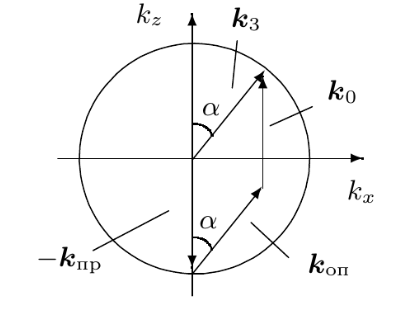
\includegraphics[width=0.6\linewidth]{img5.png}
\caption{Ориентация волновых векторов при восстановлении действительного изображения}
\label{img5}
\end{figure}

Если предмет рассеивает падающую на него волну под небольшими углами, а волновые векторы $\mathbf{k}_{\text{пр}}$ мало отличаются от $(0, 0, k)$, то поле $f_3(\mathbf{r})$ связано с действительным изображением предмета. Для наблюдения этого изображения нужно расположить голограмму перпендикулярно лазерному лучу и рассматривать её под углом $\alpha$, т.е. под тем же углом, под которым падала опорная волна. Изображение возникает между голограммой и глазом наблюдателя. Если набор волновых векторов $\mathbf{k}_0$ значительно отличается от $(0, 0, k)$, то удовлетворить условиям (7)-(8) одновременно для всех $\mathbf{k}_{\text{пр}}$ не представляется возможным, поэтому качество действительного изображения заметно хуже, чем качество мнимого изображения.

\end{document}
